\documentclass[11pt,a4paper]{article}
\usepackage[T1]{fontenc}
\usepackage[utf8]{inputenc}
\usepackage[italian]{babel}
\usepackage[italian]{varioref}
\usepackage{amsmath}
\usepackage{amsfonts}
\usepackage{subfigure}
\usepackage{amssymb}
\usepackage{indentfirst}
\usepackage{graphicx}
\usepackage{floatflt}
\usepackage{float}
\usepackage{caption}
\usepackage{tikz}
\usepackage[cdot, thickqspace, squaren]{SIunits}
%\usepackage[nomargin,inline,marginclue,draft]{fixme}
\usepackage[left=2cm,right=2cm,top=2cm,bottom=2cm]{geometry}
%\newcommand{\rem}[1]{[\emph{#1}]}

%Intestazione
\usepackage{fancyhdr}
\pagestyle{fancy}
\lhead{Esperienza N.1}
\chead{Ottica 2}
\rhead{Gruppo BF}

%Dichiarazione di operatori necessari per scrivere formule e unità di misura
\DeclareMathOperator{\uV}{\mu V}
%\DeclareMathOperator{\ohm}{\Omega}
\DeclareMathOperator{\kohm}{k\Omega}
\DeclareMathOperator{\Mohm}{M\Omega}
\DeclareMathOperator{\uA}{\mu A}
\DeclareMathOperator{\us}{\mu s}
\DeclareMathOperator{\uF}{\mu F}

%comendi in prova
\newcommand{\figura}[1]{\textsf{Figura \ref{#1}}}
\newcommand{\tabella}[1]{\textsf{Tabella \ref{#1}}}
\newcommand{\equazione}[1]{\textsf{Equazione \ref{#1}}}


\author{Gruppo BF \\ \smallskip Thomas Giannoni, Valerio Lomanto, Roberto Ribatti}
\title{Esperienza N.1 \\Ottica 2}
\date{17 febbraio 2017}
\begin{document}
\maketitle

\begin{abstract}
In quest'esperienza si è sfruttato il fenomeno dell'interferenza per determinare la frequenza di emissione di diverse sorgenti luminose.
\\L'esperienza si suddivide in due parti: nella prima si vuole stimare
la lunghezza d'onda di una laser He-Ne sfruttando la diffrazione sulla scala
graduata di un calibro; nella seconda viene impiegato un interferometro di
Michelson per stimare la lunghezza d'onda della riga verde dello
spettro di una lampada al mercurio.
\end{abstract}

%\newpage

%\tableofcontents %dovrebbe fare l'indice
\newpage
\part{Misura della lunghezza d'onda di un laser HE-NE } \label{part:Ottica_1A}
\section{finalità}
Lo scopo di questa sezione è la misura della lunghezza d'onda,$\lambda$,di 
un laser HE-NE attraverso lo studio delle figure di diffrazione prodotte 
dal reticolo.
\section{Strumentazione}
La strumentazione impiegata nella prima parte dell'esperienza consta di:
\begin{list}{$\cdot$}{}
\item \textbf{un calibro ventesimale}, del quale abbiamo impiegato la scala gradata del righello come reticolo
di diffrazione  (passo reticolare $1$ 
$[mm]$)%non ricordo con precisione.
\item \textbf{un laser HE-NE}, quale sorgente del fascio di radiazione,di ci vogliamo calcolare la lunghezza 
d'onda.
\item \textbf{uno specchio},col quale orientare il fascio emesso dal laser.
\item \textbf{uno schermo} ove vedere la diffrazione prodotta dal reticolo.
\item \textbf{un metro a nastro},risoluzione $1$ $[cm]$,col quale misurare la distanza tra il reticolo di 
diffrazione e lo schermo.
\item \textbf{un righello},risoluzione $1$ $[mm]$ per misurare l'altezza dei vari spot 
luminosi emesso sullo schermo.

\end{list}
\bigskip


\begin{figure} [!h]
	\centering
	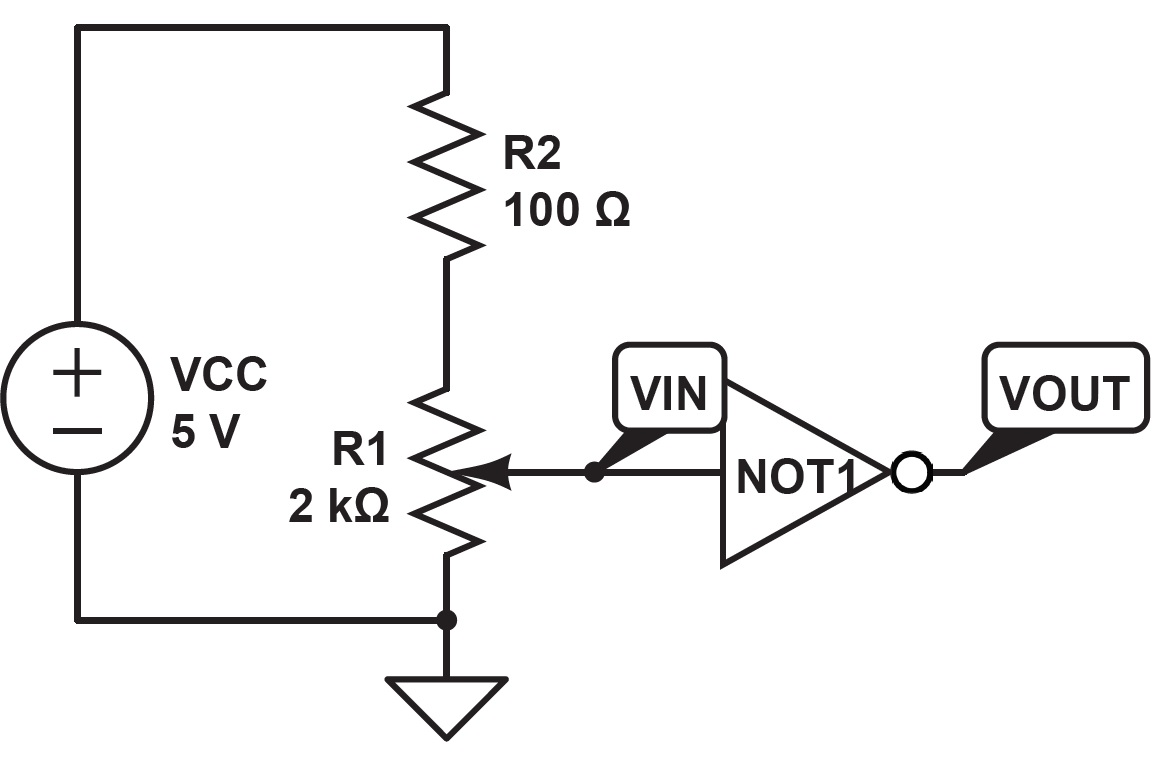
\includegraphics[width=0.9\textwidth]{./pictures/immagine1}
	\caption{Schema dell'apparato impiegato per la misura $\Lambda$.}
	\label{fig:schema_appar}
\end{figure}
Si riporta in \textbf{figura \ref{fig:schema_appar} }uno schema dell'apparato sperimentale impiegato. 
\section{Svolgimento delle misure}
Come prima cosa è stata effettuata la calibrazione dell'apparato 
strumentale:
\begin{itemize}
	\item Si sono allineati raggio laser, reticolo di diffrazione e schermo, attraverso le viti di regolazione dello specchio abbiamo fatto incidere il raggio in maniera radente sulla scala del calibro, questo è necessario per osservare sullo schermo un numero significativo di spot luminosi, essendo $\lambda \ll d$.
	\item Si è proceduto a determinare il punto \textbf{zero}: la proiezione dell'asse della scala del calibro sullo schermo. Rispetto a questo punto sono state misurate le distanze delle frange di interferenza e la distanza $D$ dello schermo dal reticolo. Per determinare la posizione di questo punto si è preso il punto medio tra lo spot luminoso del fascio diretto del laser (ben visibile senza calibro) e quello del fascio riflesso sul calibro.
\end{itemize}
La relazione che lega le grandezze in gioco è:
$$ sin (\theta_m) =-\frac{\lambda}{d}m+sin (\theta_i)$$
Dove $m$ indica il numero della frangia di diffrazione, $d$ è il passo reticolare, $\theta_i$ e $\theta_m$ sono rispettivamente l'angolo di incidenza e l'angolo della frangia $m$-esima, $D$ è la distanza dello schermo dal reticolo.

Si è proceduto alla misura della distanza $D$ tra il punto \textbf{zero} prima determinato e il reticolo di diffrazione, la dimensione del fascio laser che incide radente sulla scala del calibro non è trascurabile, ha infatti un'estensione di $\sim \unit{10}{\centi\meter}$, bisogna tenerne conto nella stima dell'incertezza.

Il risultato della misura è stato $D = \unit{209 \pm 3}{\centi\meter}$.

Conoscendo $D$ e dalla misura delle distanze delle frange di diffrazione dal punto zero è possibile determinare i $\theta_m$ e procedere ad un fit lineare di $sin(\theta_m)$ in funzione di $m$ con coefficiente angolare $-\lambda/d$ e intercetta pari a $sin(\theta_i$.)

Le misure effettuate sono riportate in \tablename{ \ref{\{data}} Il fit eseguito fornisce i seguenti risulati;
\begin{figure}[H]
	\begin{minipage}{0.25\textwidth}
		\begin{tabular}{l}
			$\lambda/d = \unit{63.38 \pm 0.07}{\micro\meter}$ \\
			$\theta_i = (89.56 \pm 0.03) $\\
			$corr(\lambda/d,\theta) = -0.77$\\
			$\chi^2 /\text{ndof} = 21.3 / 17 $\\
			$p_{val} = 0.21$
		\end{tabular}
	\end{minipage}
	\begin{minipage}{0.8\textwidth}
		\centering
		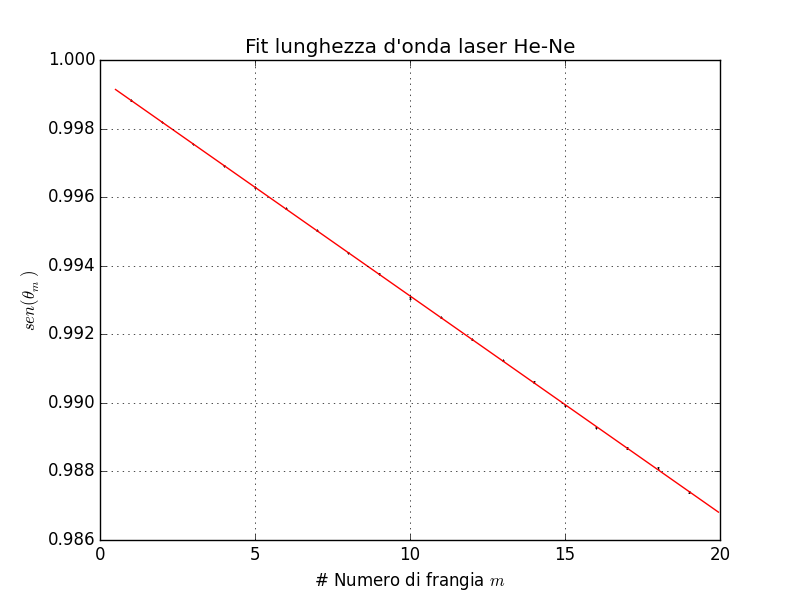
\includegraphics[width=\textwidth]{./pictures/fit_He-ne.pdf}
	\end{minipage}
\end{figure}

dal quale segue $\lambda = \unit{633.8 \pm 0.7}{\nano\meter}$.
\section{Note e osservazioni}
Come espresso nelle sezioni precedenti la misura richiede alcuni accorgimenti:
si osserva che il punto di incidenza 
presenta un estensione non trascurabile sul calibro.
Si è quindi ritenuto opportuno misurare $D_{min}$ e $ D_{max}$
assumendo come valore di $D$ il valore medio. Si è deciso, ai fini del fit, di considerare comunque un'incertezza di $\unit{1}{\milli\meter}$, cioè la risoluzione dello strumento poichè l'errore dovuto alla dimensione del punto di incidenza è un errore sistematico.

Si è inoltre assunto che l'incertezza sul passo
reticolare $d$ fosse trascurabile rispetto alla precisione della misura, inoltre tale errore sarebbe un errore di calibrazione pertanto dovrebbe essere trattato separatamente da quelli stocastici e 
escluso dagli errori impiegati nel fit lineare.
\part{Interferometro di Michelson }

\section{Strumentazione}
La strumentazione impiegata in questa sezione  si 
compone di un interferometro di Michelson e da una fotocamera,
impiegata come ausilio per il conto delle frange di interferenza.

L'interferometro di Michelson è composto da:
\begin{list}{}{}
\item \textbf{una sorgente}, costituita da un \textbf{laser HE-NE}, 
quale sorgente di $\lambda$ nota,
per la taratura del sistema; da una \textbf{lampada al mercurio} quale 
sorgente di cui analizzare la riga di emissione più intensa; una lampada
di luce bianca;
\item \textbf{un beam splitter} per dividere la radiazione della sorgente
in 2 fasci coerenti che percorreranno i
due bracci dell'interferometro;
\item \textbf{due specchi} posti al termine dei bracci 
dell'interferometro.;
\item \textbf{uno schermo} dove osservare l'interferenza alla ricombinazione dei 2 
fasci uscenti dall'interferometro e generati dal laser HE-NE.
\item \textbf{un filtro verde}, necessario per selezionare 
la riga verde dell'emissione della lampada a mercurio.
\end{list}
\bigskip

Si riporta in \figurename{ \ref{fig:schema_appar2}} uno schema dell'apparato sperimentale impiegato. 
\begin{figure} [H]
	\centering
	\includegraphics[scale=0.5]{./pictures/immagine2}
	\caption{Schema dell'apparato impiegato per la misura.}
	\label{fig:schema_appar2}
\end{figure}

\section{Misura di $\lambda_{Hg}$ per la riga verde della lampada a mercurio}
\subsection{Taratura del sistema}
Per effettuare la misura della lunghezza d'onda 
della riga verde di emissione della lampada
a mercurio, l'apparato necessita di una fase 
preventiva di taratura.

In questa fase si cerca di porre in relazione la differenza 
di cammino ottico $\Delta x$ allo spostamento letto 
sul micrometro $\Delta L$,
ovvero il fattore di demoltiplica della leva $y$.
Per effettuare tale calibrazione abbiamo 
montato una sorgente di  $\lambda$ nota,nello specifico un laser
HE-NE di $\lambda_{He-Ne}=633 [nm]$.
Posta la scala del micrometro, in corrispondenza dello zero,
attraverso il meccanismo posto su M2 abbiamo allineato i fasci 
uscenti dai de bracci dell'interferometro;
dopodiché abbiamo preso 
come riferimento un punto e abbiamo osservato allo spostarsi dello 
specchio M1 il numero di frange che si vedono 
passare al variare di $\Delta L$.
Essendo valida \smallskip
\begin{equation}\label{eq:lambda}
2 \cdot \Delta x = m \cdot \lambda
 \end{equation}
 \smallskip
dove $m$ è il numero di frange osservate, possiamo ricavare 
il fattore di demoltiplica $y=\frac{\Delta x}{\Delta L}$.

Essendo possibile che in fase di conteggio si perdano 
alcune frange di interferenza, abbiamo registrato il passaggio delle frange attraverso la fotocamera 
per effettuare successivamente il conteggio; si è trovato\\
$m=73 \pm 0.5 \qquad \text{corrisponde a}\qquad \Delta L =120\pm 3 [\mu m]$
\\
Se ne ricava pertanto come valore di $y= 0.193	\pm	3$.
Il valore di m è stato dato con un incertezza di mezza frangia poiché, sebbene il conteggio delle frange "intere" sia stato esatto (grazie alla registrazione), non sappiamo con esattezza quanto fossimo distanti dal vedere la frangia successiva quando ci siamo fermati.
Stimiamo un tale errore per la distanza percorsa dalla vite micrometrica 
in virtù dell'aver scelto di fermarci proprio quando la misura sembrava essere il più precisa possibile,
dunque riteniamo di avere un'incertezza decisamente minore della mezza tacca.
\subsection{Misure e procedimento}
Per effettuare la misurazione di $\lambda_{Mg}$
abbiamo sostituito il laser HE-NE con 
lampada a mercurio.
Essendo lo spettro di emissione della lampada 
composto di numerose righe
abbiamo frapposto un filtro tra la sorgente e il beam splitter,
così da osservare esclusivamente la riga verde,la più intensa.
Essendo la nostra radiazione non abbastanza intensa da essere 
proiettata sullo schermo il conteggio delle frange di interferenza
è stata effettuata registrando direttamente dall'uscita del beam-splitter; 
per semplificare il conteggio abbiamo 
posto come riferimento una punta sul nostro filtro ed effettuato il conteggio 
dalla registrazione come nella nella fase di calibrazione.
Osservando il $\Delta L$ corrispondenti a $m$ frange di
interferenza applicando l'\equazione{eq:lambda} e dalla conoscenza di $y$ 
possiamo ottenere $\lambda$;
nella fattispecie avendo osservato che
\\
 $m=71 \pm 1\text{corrisponde a}\qquad \Delta L =100\pm 3 [\mu m]$
 \\
 $m=72 \pm 3\text{corrisponde a}\qquad \Delta L =100\pm 3 [\mu m]$
 \\
impiegando l'\equazione{eq:lambda} si ottiene $\lambda_{Hg}=544\pm 5$ che 
risulta essere in accordo col valore atteso 	
$\lambda_{attesa}\sim 546 [nm]$
\section{Frange di interferenza con luce bianca}
Per osservare le frange di interferenza con la luce bianca
abbiamo inizialmente posto uno spessore metallico su M1.
Abbiamo allineato nuovamente il sistema impiegando il laser;
dopodiché spostando M1 abbiamo ritrovato le frange di interferenza
per la lampada a mercurio e il filtro verde; così da rendere 
la differenza tra i due bracci dell'interferometro quasi nulla.
Spostando ulteriormente M1 abbiamo ottenuto le frange di interferenza per
la luce bianca,si riporta l'osservazione in 
\bigskip
\begin{figure} [!h]
	\centering
	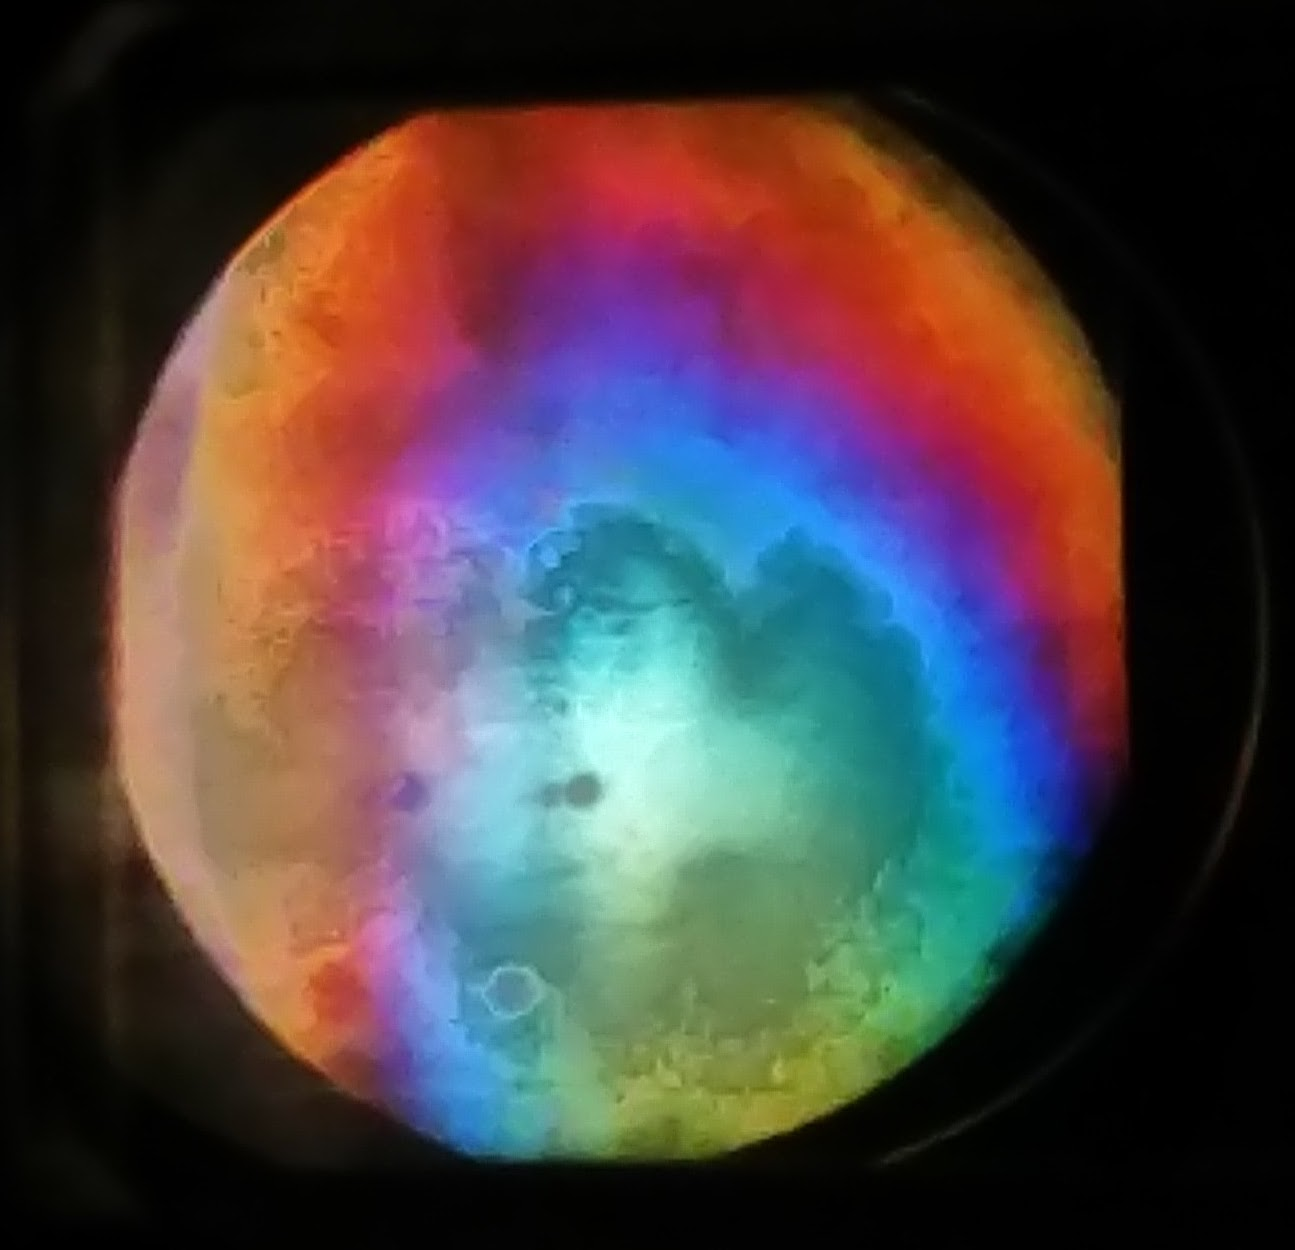
\includegraphics[width=0.9\textwidth]{./pictures/frange.jpg}
	\caption{frange di interferenza per luce bianca.}
	\label{fig:frangeb}
\end{figure}
\bigskip
\figura{fig:frangeb}.
Una ragione per cui il cammino ottico sui
de bracci dell'interferometro debba essere all'incirca uguale è
 il fatto che in tale configurazione l'interferenza non risulta
dipendente da $\lambda$: infatti con una sorgente così lontana
dall'essere monocromatica qualsiasi dipendenza significativa dalla
lunghezza d'onda risulterebbe nell'assenza di fenomeni apprezzabili a occhio nudo,
poiché le diverse componenti dello spettro della sorgente darebbero una distribuzione di frange
molto diversa, e la sovrapposizione di queste apparirebbe essenzialmente uniforme.
\section{Note e osservazioni}
In questa sezione la principale difficoltà
riscontrata in questa esperienza risulta essere il conteggio del
numero di frange di interferenza.
Essendo in caso di movimenti bruschi facile
perdere il conto delle frange,sia in fase di 
calibratura che in fase di misura, abbiamo deciso di registrare 
il passaggio delle bande attraverso una fotocamera digitale,
avendo cura di iniziare e terminare la registrazione rispettivamente qualche 
secondo prima dell'inizio dello spostamento di M1
e qualche secondo dopo la fine del movimento.
Questo accorgimento ha permesso di poter fare il conteggio a seguito
potendo regolare la velocità del video;riducendo conseguentemente l'incertezza 
sul conteggio delle frange.
Un ulteriore sistema che abbiamo usato per diminuire l'influenza 
di eventuali errori di conteggio riguarda il numero di frange che andiamo a 
considerare;
Abbiamo noi ritenuto un numero congruo $m> 50$
poiché al crescere di $m$ sia l'incertezza su $\Delta L$ che l'eventuale 
errore su $m$ risulta avere un influenza minore.

L'impiego della fotocamera digitale per la lampada al mercurio,e l'analisi del
relativo filmato, 
hanno posto in evidenza l'esistenza di un rumore di frequenza $50 Hz$ o 
suoi multipli; tale rumore infatti spariva impostando $50 Hz$ come velocità di shutter della fotocamera.
Si ritiene pertanto che questo rumore sia dovuto  ad un accoppiamento con 
la tensione di rete. 

Qualora non indicato diversamente anche in questa sezione le incertezze sono 
state propagate
con metodo della somma in quadratura.
\newpage
\appendix
\section{Appendice} \label{sec:Appendice}

\begin{table}[H]
	\centering
\begin{tabular}{c|c|c} 
	m & distanza [cm]\\
	\hline
	0& 6.90 $\pm$ 0.10\\
	1& 17.05 $\pm$ 0.05\\
	2& 19.50 $\pm$ 0.05\\
	3& 21.55 $\pm$ 0.05\\
	4& 23.35 $\pm$ 0.05\\
	5& 24.95 $\pm$ 0.05\\
	6& 26.40 $\pm$ 0.05\\
	7& 27.80 $\pm$ 0.05\\
	8& 29.15 $\pm$ 0.05\\
	9& 30.35$\pm$ 0.05\\
	10& 31.65 $\pm$ 0.05\\
	11& 32.65 $\pm$ 0.05\\
	12& 33.75 $\pm$ 0.05\\
	13& 34.75 $\pm$ 0.05\\
	14& 35.75 $\pm$ 0.05\\
	15& 36.80 $\pm$ 0.05\\
	16& 37.75 $\pm$ 0.05\\
	17& 38.60 $\pm$ 0.05\\
	18& 39.45 $\pm$ 0.05\\
	19& 40.40 $\pm$ 0.05\\
\end{tabular}
\captionof{table}{Dati raccolti}
\label{data}
\end{table}



\end{document}



